%TEX root = ../dissertation.tex

\chapter{Background}
\label{chapter:background}

\section{Early attempts at multi-game playing}



\subsection{Hoyle}
A system developed in the 90’s, using a training scheme called lesson and practice, where lessons are games played against an expert and practice is self-playing. Predates GDP and was developed for 2-player games. The system used a set of game independent Advisers, each specialized in a game aspect such as position. These Advisers could recommend moves that could then be chosen by higher tier advisers. There were 3-tiers, depending on specialization:

\begin{enumerate}

\item [1st.] These Advisers specialized in immediate consequences: they performed very shallow searches to avoid things like instant loss moves. These decisions were final.

\item [2nd.] Advisers in this tier chose moves according to certain goals. These decisions were also final.

\item [3rd.] Advisers in the last tier differed from the first tiers in an important way: The decision of each Adviser wasn’t final, the final decision was decided by a process similar to taking a vote between the Advisers in this 3rd tier. Advisers votes were weighted in accordance to the lesson and practice results: Advisers that were more often correct during the training stage received bigger weights. 

\end{enumerate}
This process of weighting the Advisers was crucial to the performance of the system and could even be worse than a random player if done incorrectly. If none of the 3rd tier advisers were even remotely related to the game being played the results would also be disappointing. Having a varied pool of Advisers was for this reason vital but they were never, by definition, general enough. Hoyle was tested in 18 two-player board games, its potential in complex games was never verified.

\section{The basics of General Game Playing}

General Game Playing is a project of the Stanford Logic Group of Stanford University, California, which aims to create a platform for \gls{GGP}.
Since 2005, there have been annual \gls{GGP} competitions at the AAAI Conference.


A \gls{GGP} match consists of 3 major components:
\begin{itemize}
\item Game Description: The game rules, in \gls{GDL}.

\item Game Manager: This system acts as a referee and manages communication with the players and other systems like graphics for the spectators. \textit{State Data} is usually part of the Game Manager.

\item Players: Players are the most interesting component of a \gls{GGP} game, they need.

\end{itemize}

\begin{figure}[h]
	\centering
    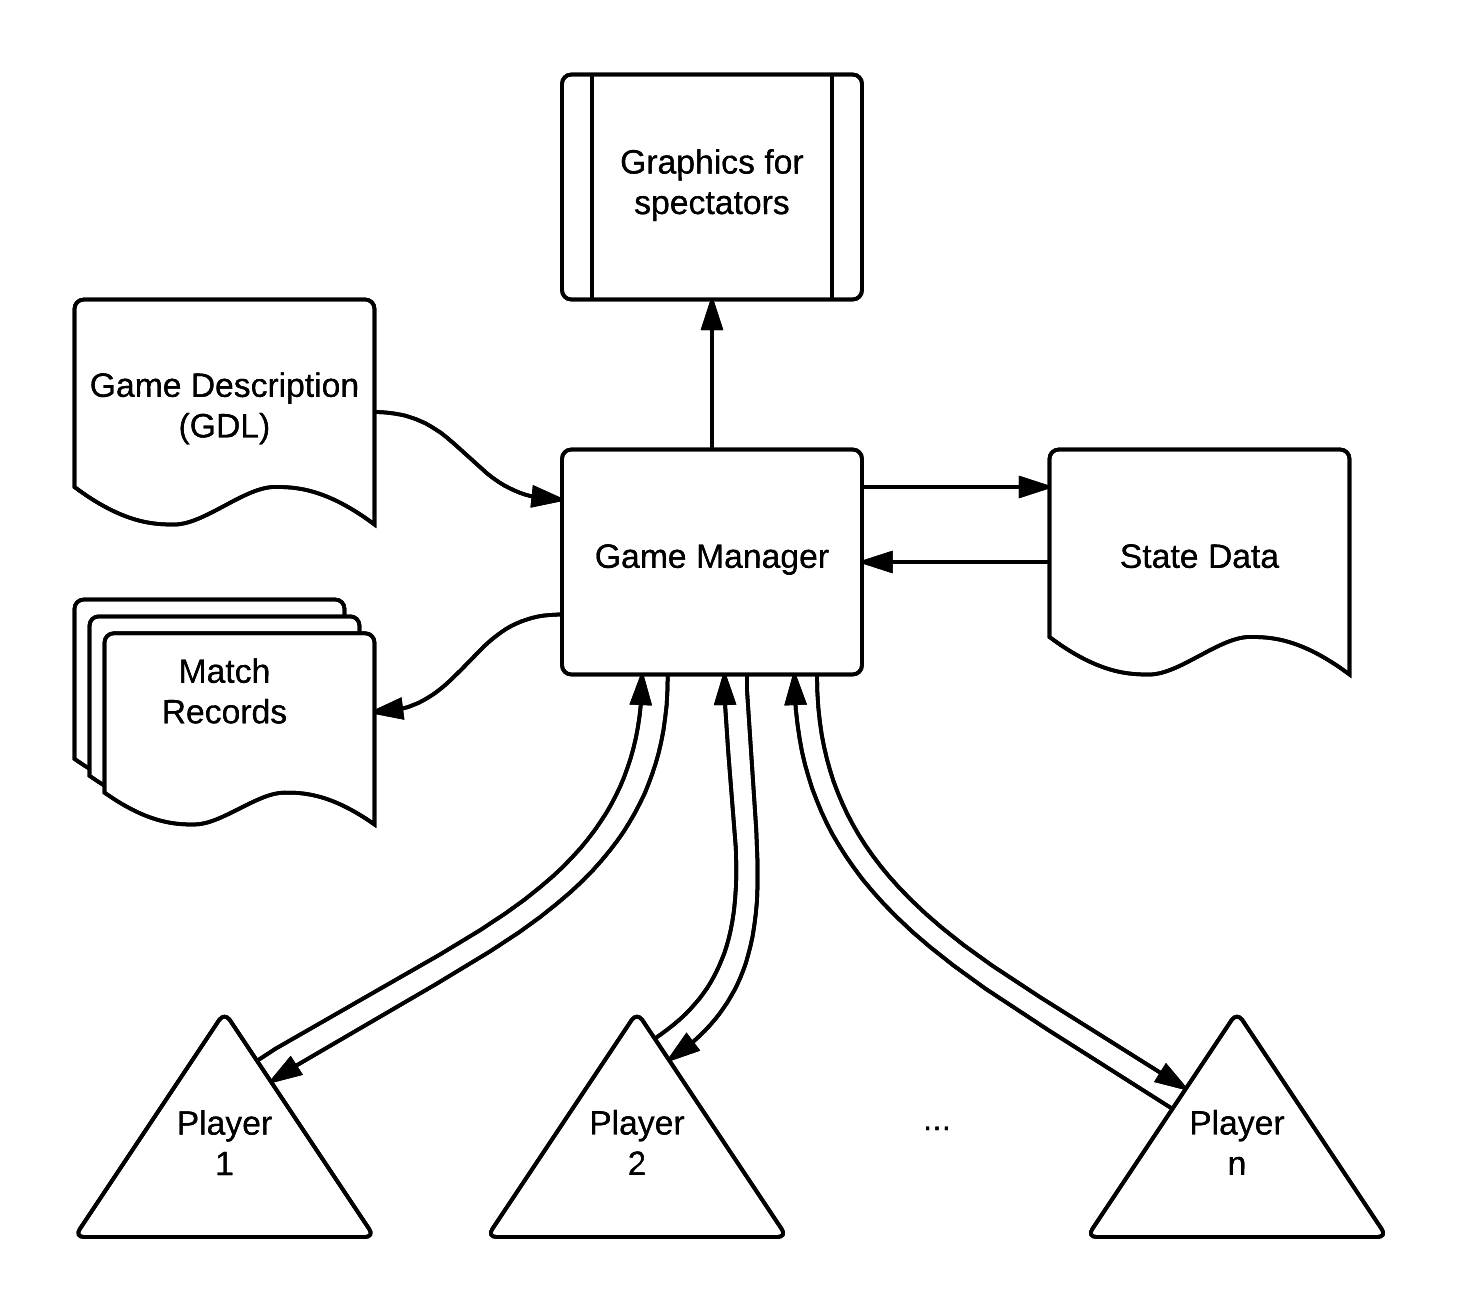
\includegraphics[scale=0.8]{images/GGPgamesetup.png}
    \caption{Match Components}
    \label{fig:match components}
\end{figure}

At the beginning of a match, the Game Manager sends all Players a match identifier, the game description, the role of each player and the time limits (for preparation (\textit{startclock}) and for each round (\textit{playclock})).

The match commences, after all players respond, with the Game Manager requesting a move from all players. Each round ends when all players send their moves or the time limit runs out (a random legal move is chosen for players that don't respond in time), after which the Game Manager will send each player another request along with all moves taken in the previous round.


\subsection{Game Description Language}
The \gls{GDL} is the standard way of describing games in the \gls{GGP} community.
\gls{GGP} players interpret the language using something called a \textit{Reasoner}. Choosing a good way of interpreting the game rules is one of the keys to performance and so many players develop their own custom \textit{reasoners}.

It can describe any finite deterministic move-based strategy game with an arbitrary number of players (most board games). GDL-II is an extension that has been made to allow for probabilistic games and incomplete information, like most card games.

Both GDL and GDL-II are variants of Datalog (query and rule language similar to prolog) and use first order logic.
Since GDL is a very conceptual description of the rules their interpretation is very computationally expensive. Choosing a good way of doing this interpretation (components that do this are called reasoners) is therefore very important to player performance, even in the recent years.

An example of tic tac toe described in GDL with some syntax explanation can be seen in \ref{appendix:gdl_example}

\subsection{Game Manager}
The purpose of the Game Manager is to be a single source of truth about what's happening in a match, and verify all moves taken by players. It must be able to interpret \gls{GDL}, to verify these moves

Players communicate their moves to the Game Manager (via HTTP), who checks the validity of the moves. A random legal move is chosen if a player chooses an illegal move or doesn't respond in time.

It should also provide a way of archiving the match history (all game states and moves taken) and other useful features like an interface for spectating.

\subsection{Game Player}
Game Players are systems that can interpret a \gls{GDL} game description, communicate with the Game Manager and devise strategies, to maximize their result in a certain game.

Game Players are, of course, the most interesting part of any \gls{GGP} match. Their aim is to be as general as possible while also having reasonably good performance in any game, which is a surprisingly difficult feat. Suffice it to say, sophisticated AI techniques like heuristics are very hard to successfully apply in a general, domain independent, way. So far, 
The most relevant techniques are discussed in chapter \ref{chapter:state_of_the_art}.



